\documentclass[8pt, english]{article}
%%%%%%%%%%%%%%%%%%%%%%%%%%%%%%%%%%%%%%%%%%%%%%%%%%%%%%%%%%%%%%%%%%%%%%%%%%%%%%%%%%%%%%%%%%%%%%%%%%%%%%%%%%%%%%%%%%%%%%%%%%%%
\usepackage{latexsym,amssymb,amsfonts,hyperref,fullpage,graphicx, float,adjustbox}
\usepackage[fleqn]{amsmath}
\usepackage{multicol}
\usepackage{lastpage,listings}
\usepackage[hang, small,labelfont=bf,up,textfont=it,up]{caption} % Custom captions under/above floats in tables or figures
\usepackage{placeins}
\usepackage{adjustbox}
\usepackage[toc,page]{appendix}
\usepackage{tabulary}
\usepackage[landscape,margin=0.25in]{geometry}
%\usepackage[landscape]{geometry}
\title{Gabby Cheat Sheet} 
\makeatletter
\renewcommand{\section}{\@startsection{section}{1}{0mm}%
                                {-1ex plus -.5ex minus -.2ex}%
                                {0.5ex plus .2ex}%x
                                {\normalfont\large\bfseries}}
%\renewcommand{\subsection}{\@startsection{subsection}{2}{0mm}%
%                                {-1explus -.5ex minus -.2ex}%
%                                {0.5ex plus .2ex}%
%                                {\normalfont\normalsize\bfseries}}
%\renewcommand{\subsubsection}{\@startsection{subsubsection}{3}{0mm}%
%                                {-1ex plus -.5ex minus -.2ex}%
%                                {1ex plus .2ex}%
%                                {\normalfont\small\bfseries}}
\makeatother
\begin{document}
\begin{multicols}{4}
\raggedright
\footnotesize

\subsection*{Projective Geometry}
Homography maps original image to new frame 	
each point has some lambda. Can use vanishing points as points 
%\FloatBarrier
%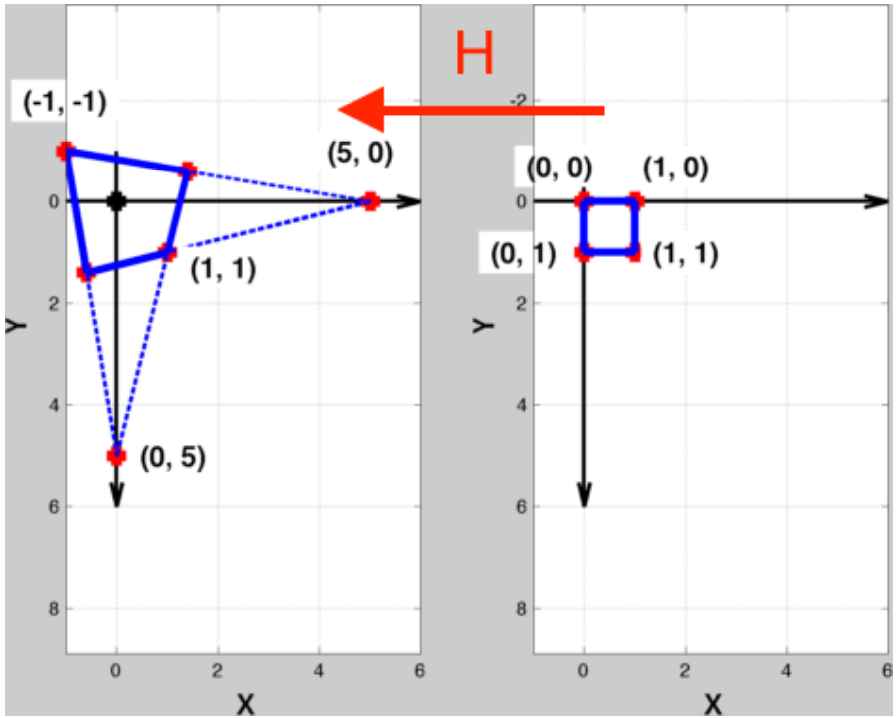
\includegraphics[width = \linewidth]{cheat1.png}
\begin{flalign*}
\lambda_i x_i'  = Hx_i \\ 
\lambda_1  \begin{pmatrix}
-1 \\ -1 \\ -1
\end{pmatrix} = H \begin{pmatrix}
0 \\ 0 \\ 1
\end{pmatrix} <-- h3  \\ 
\lambda_2 \begin{pmatrix}
5 \\0 \\ 1
\end{pmatrix} = H \begin{pmatrix}
1 \\ 0 \\ 0
\end{pmatrix} = \begin{pmatrix}
5 \lambda_2 \\ 0  \\ \lambda_2 
\end{pmatrix}\\
ect ..\\
H = \begin{pmatrix}
5 \lambda_2 & 0  & -1 \\ 
0 &  5\lambda_3  & -1 \\ 
1 & 1 & 1\\
\end{pmatrix}
\end{flalign*}
\subsection*{Homogenous Coordinates of line }
\begin{flalign*}
L' = (H^{-1})^{-T} L  \\ 
L' = H^T L \\
\text{ Homogenous form of L for line at infinity}\\
l = \begin{pmatrix}
		0 \\ 0 \\ 1 
\end{pmatrix}
\end{flalign*}
\subsection*{Vanishing Points}
given an image , find two lines on image that should be parallel in real life, but intersect in the image. a and b are two points on the top line, d and e are two points on bottom line  then 
\begin{flalign*}
v = (\begin{vmatrix}
a \\ 1
\end{vmatrix} \times \begin{vmatrix}
b \\1 
\end{vmatrix})  \times  (\begin{vmatrix}
d \\ 1
\end{vmatrix} \times \begin{vmatrix}
e \\1 
\end{vmatrix}) \\
\textbf{CROSS RATIO DOES NOT } \\
\textbf{CHANGE IN HOMOGRAPHIC }\\
\textbf{TRANSFORMATION}\\
\frac{||a - c|| ||b - v||}{||b - c|| || a - v||}\\
\end{flalign*}

\subsection*{Homography Estimation}
\begin{align*}
x_2 = H x_1 \\
x_2 \times H x_1 = 0 \\ 
\begin{bmatrix}
0 & -1  & v \\  1 & 0 & -u \\  -v &  u & 0
\end{bmatrix} \begin{bmatrix}
x_1^{T} & \mathbf{0}_{1x3} &  \mathbf{0}_{1x3} \\ 
\mathbf{0}_{1x3} & x_1^{T} & \mathbf{0}_{1x3} \\ 
\mathbf{0}_{1x3} & \mathbf{0}_{1x3} & x_1^{T}
\end{bmatrix} \begin{bmatrix}
h_1^{T} \\ h_2^{T} \\ h_3^{T}
\end{bmatrix}\\
\begin{bmatrix}
\mathbf{0}_{1x3}  & -x_1^{T}  & v_2 x_1^{T} \\  x_1^{T} & \mathbf{0}_{1x3} & -u_2 x_1^{T} \\  -v_2 x_1^{T} &  u_2 x_1^{T} & \mathbf{0}_{1x3} 
\end{bmatrix} \begin{bmatrix}
h_1^{T} \\ h_2^{T} \\ h_3^{T}
\end{bmatrix}\\
\text{ This is in the form $ Ax = 0 $} 
H = \begin{bmatrix}
h_1 \\ h_2 \\ h_3 
\end{bmatrix}\\
r_1 = K^{-1}h_1 / || K^{-1} h_1 || \\
r_2 = K^{-1} h_2 / || K^{-1}h_2 || \\
r_3 = r_1 \times r_2 \\
t = K^{-1} h_3 / || K^{-1}h_1|| \\
\end{align*}
\subsection*{Skew Matrix!}
\begin{align*}
\begin{bmatrix}
0 & -a_3  & a_2 \\  a_3 & 0 & -a_1 \\  -a_2 &  a_1 & 0
\end{bmatrix}
\end{align*}
2d cross product 
\begin{align*}
 x \times  y = x_1 y_2 - x_2 y_1
\end{align*}
3d cross product 
\begin{align*}
u \times v = (u_2 v_3 - u_3 v_2) \mathbf{i}\\
 + (u_3 v_1 - u_1 v_3) \mathbf{j} + (u_1 v_2  - u_2 v_1) \mathbf{k}\\
\text{as column vectors} \\
\begin{bmatrix}
 (u_2 v_3 - u_3 v_2)\\
  (u_3 v_1 - u_1 v_3) \\
  (u_1 v_2  - u_2 v_1)
\end{bmatrix}
\end{align*}
\subsection*{Rotation Matricies}
Rotations composed by in order by multiplying on the left
example :  
\begin{flalign*}
R_3 = R_2*R_1
\end{flalign*}

\subsection*{Axis Angle}
rotation vector is r , given two random vector a and b and some angle between them $\alpha$ \\
\begin{flalign*}
\pmb{k} = \frac{\pmb{a} \times \pmb{b}}{|a| |b| \sin \alpha}\\
\pmb{r} = \theta \pmb{k}\\
\text{rodrigues formula}\\ 
\text{k is unit vector for }\\
\text{ axis of rotation}\\
\text{ which v rotates about theta} \\ 
\pmb{v_{rot}} =  \pmb{v} \cos \theta + (\pmb{k} \times \pmb{v} ) \sin \theta\\ + \pmb{k} (\pmb{k} \cdot \pmb{v})  ( 1- \cos \theta)\\
\textbf{Axis angle to Rotation Matrix} \\
K = \text{ matrix cross product with v}\\
 K = \begin{pmatrix}
 0 & -k_3	& k_2 \\  k_3 & 0 &  -k_1 \\ -k_2 &  k_1 & 0 
\end{pmatrix}   \\
R = I + (\sin \theta)K  + (1 - \cos \theta) K^2
\end{flalign*}

\subsection*{Quaternions}
\begin{flalign*}
  ijk = -1  | ij = k | jk = i | ki = j \\ 
  q = \cos \frac{\theta}{2} +( u_x \mathbf{i} + u_y \mathbf{j} + u_z \mathbf{k}) \sin \frac{ \theta}{2}\\
  q  = \begin{bmatrix}
  s , & v 
  \end{bmatrix} s \epsilon \mathbb{R}  \\  
  q = \begin{bmatrix}
  s, & x\mathbf{i} & y \mathbf{j} & z\mathbf{k}\\
 \end{bmatrix}\\
  q_a q_b = [s_a, \mathbf{a}][s_b, \mathbf{b}] \\ 
  = [s_a s_b - \mathbf{a} \cdot \mathbf{b}, s_a \mathbf{b} +s_b \mathbf{a} + \mathbf{a} \times \mathbf{b}] 
\end{flalign*}
\subsection*{Camera Extrinsic Paramaters}
 World to Camera formula 
 \begin{flalign*}
 X_c = \begin{bmatrix}
 R & t 
 \end{bmatrix} X_w \\
 \text{Cameras world position is $-R^{T} t $ }\\
 \text{Rotation is $ R^{T}$} 
 \end{flalign*}
 \subsection*{Radial Distortion}
  \begin{flalign*}
  r = || x_{ideal}||\\
  u_{img} = u_{ideal} + \\
  (u_{ideal}  - p_x ) [k_1 r^2 + k_2 r^4]\\
  v_{img} = v_{ideal} +\\ 
  (v_{ideal}  - p_y ) [k_1 r^2 + k_2 r^4]\\
  \begin{bmatrix}
  (u_{ideal}  - p_x ) r^2 &  (u_{ideal}  - p_x ) r^4 \\
  (v_{ideal}  - p_y ) r^2 &  (v_{ideal}  - p_y ) r^4 \\
  \end{bmatrix} \\
  = \begin{bmatrix}
  u_{img} -u_{ideal} \\
  v_{img} - v_{ideal}
  \end{bmatrix}
  \end{flalign*}
 \subsection*{Epipolar}
 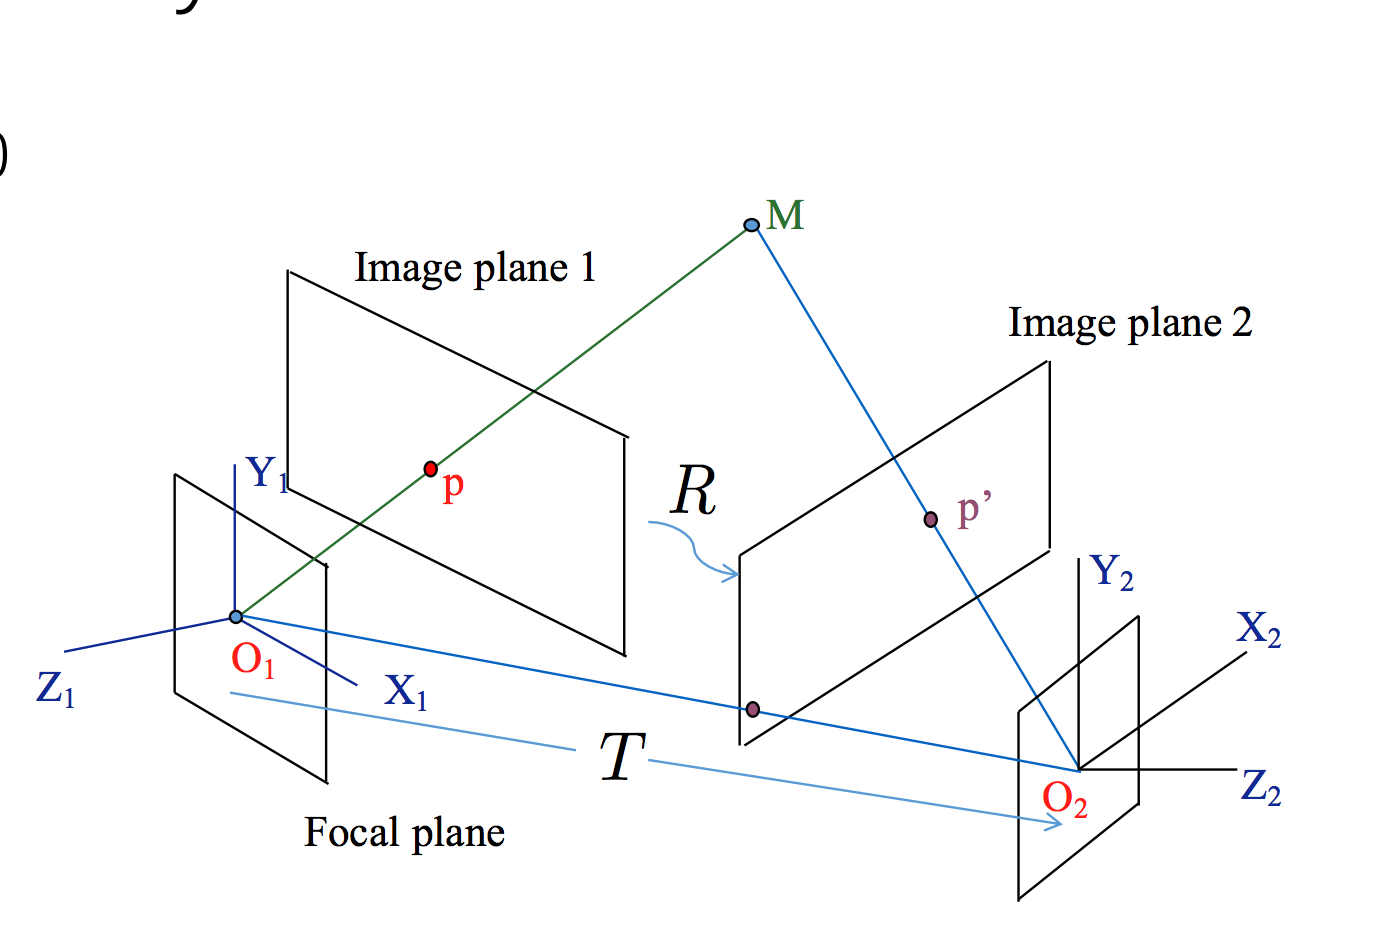
\includegraphics[scale = .3, width = \linewidth]{epipolar.png} 
 \begin{flalign*}
 \textbf{Essential Matrix} \\ 
 P_{2}^{T} E P_{1} = 0  <-- svd \\ 
 E = RT\\
 \textbf{Fundamental Matrix} \\ 
 p_{2}^{T} F p_{1}  = 0 \\
 F =  K_{2}^{-T} E K_{1}^{-1} \\ 
 \text{Epipolar Line} \\
 p_{2} = p_{0} , p_{0}^{T}Fp_{1} = 0 \\ 
 \textbf{Epipole} \\
 p_{2}^{T} F= 0 \\ 
 Fp_{1} = 0 \\
 \text{if we have$ R_1 , R_2	, t_1 ,t_2, K_1,K_2 $} \\ 
 R = R_{2}R_{1}^{T} \\
 T = t_1 - (R_{1}R_{2}^{T}t_2 ) \\
  \end{flalign*}
\subsection*{Param Estimation}
\begin{align*}
K[R|t] \begin{bmatrix}
X \\ 1 
\end{bmatrix} = P \begin{bmatrix}
X \\1 
\end{bmatrix} 
u = P_1\begin{bmatrix}
X \\1 
\end{bmatrix}\\
v = P_2\begin{bmatrix}
X \\1 
\end{bmatrix}\\ 
w = P_3 \begin{bmatrix}
X \\1 
\end{bmatrix}\\ 
\end{align*}
Non Linear Triangulation\\
\begin{align*}
J = \begin{bmatrix}
\frac{w\frac{\partial u}{\partial X} - u \frac{\partial w}{\partial X}}{ w^2} \\ 
\frac{w\frac{\partial v}{\partial X} - v \frac{\partial w}{\partial X}}{w^2}
\end{bmatrix}\\
\frac{\partial u}{\partial X}  =\begin{bmatrix}
P_{11} & P_{12} & P_{13} \\
\end{bmatrix}\\ 
\frac{\partial v}{\partial X}  =\begin{bmatrix}
P_{21} & P_{22} & P_{23} \\
\end{bmatrix}\\   
\frac{\partial w}{\partial X}  =\begin{bmatrix}
P_{31} & P_{32} & P_{33} \\
\end{bmatrix}
\end{align*}

PnP
\begin{align*}
\text{ given x,X,K solve for R,t} \\
\lambda \begin{bmatrix}
x\\1 
\end{bmatrix} = P \begin{bmatrix}
X \\1
\end{bmatrix}\\
\begin{bmatrix}
u\\ v \\1 
\end{bmatrix} = P \begin{bmatrix}
X \\1 
\end{bmatrix}\\
\text{ PnP} \\ 
[ R |t ] = K^{-1} P 
\end{align*}  
\subsection*{Calculate Calibration}
\begin{align*}
\text{Let $Q = [R | t]  \begin{bmatrix}
X \\1 
\end{bmatrix}$}\\
\lambda\begin{bmatrix}
x \\1 
\end{bmatrix} = \begin{bmatrix}
f_x & s & p_x  \\  0 & f_y  & p_y \\  0 & 0 & 1
\end{bmatrix} Q = 0 \\ 
\begin{bmatrix}
u\\ v \\1 
\end{bmatrix} \times 
\begin{bmatrix}
f_x & s & p_x  \\  0 & f_y  & p_y \\  0 & 0 & 1
\end{bmatrix} Q = 0 \\  
\end{align*}
\begin{flalign*}
A = \begin{bmatrix}
Q_x & Q_y & Q_z &0 &0 &0 \\ 
0&0&0&Q_y & Q_z & 0  \\ 
0 & 0 & 0 & 0 &0 &Q_z 
\end{bmatrix} \\
\begin{bmatrix}
0 & -1  & v \\  1 & 0 & -u \\  -v &  u & 0
\end{bmatrix} A
 \begin{bmatrix}
f_x \\ s \\  p_x \\ f_y\\ p_y \\ 1
\end{bmatrix} = 0 \\
\end{flalign*}
\end{multicols}
\end{document}
